%!TEX root = ../username.tex
\chapter{Are Virtual Things Real?}
\section{Definitions}
At first glance, the question, an answer to the question "virtual things real?" appears trivial. Clearly, the Pokemon in my handheld game are nothing more than a series of electromagnetic patterns. The same could be said of any sense-experience we have. 
Before we can investigate the claim "are virtual worlds real?", we must first establish what we mean by the claim. In his article \textit{The Virtual and the Real}, David Chalmers describes the term virtual as having several commonplace definitions. One common meaning of the term "virtual", claims the phrase "virtual X" means something along the lines of "as if X but not X" . On that reading, virtual reality is an unreal as-if reality, and virtual reality is no more reality than a virtual kitten is a kitten. \cite{ChalmersVR} While this definition is widely cited in dictionaries and other authoritative sources of definitions, it does not reflect the term’s contemporary definition. The advent of modern computer technology has resulted in a second widely used definition of the term virtual When used in discussions regarding computing, English speakers  tend to mean something along the lines of "a computer-based version of X" when talking about a "virtual X. Under this more contemporary description, virtual reality can be a sort of reality, just a virtual bank is a real bank (insofar as it fulfills all of the roles and functionalities we typically associate with an organization with the label of "bank"). 
For many readers, this recitation of definitions may appear pedantic. However, the dual definitions of the term "virtual" suggests that perhaps the opposition towards virtual realism is in part motivated by linguistics, just as proponents of the identity thesis in the philosophy of mind struggle with the inherent dualist bias in how English speakers and Western Philosophy think about these ideas. I will discuss this view of mine at greater length at later points in this paper, however for now I will merely say the first term should not be applied to descriptions of computer systems that instantiate via a combination of hardware and software an environment in which an agent can interact with entities described by software instructions. To apply the first term to these sorts of systems implies either confusion about the nature of these systems or an attempt to argue against virtual realism by begging the question. 
The second definition presented by Chalmers encompasses a wide array of systems and environments. These spaces range from the permanent and all-encompassing environment depicted in the 1999 science fiction movie \textit{The Matrix} to the ephemeral argumentation of the hit Android and iOS game, \textit{Pokemon Go}. In \textit{Matrix as Metaphysics}, Chalmers argues that "if we are in a Matrix, most of our ordinary beliefs (e.g. that there are tables) are true: if we discovered that we are in a Matrix, instead of saying that there are no tables, we should say instead that tables are computational objects made of bits". Chalmers describes this view as \textit{digitalism}, the claim that: \begin{enumerate}
	\item Virtual objects really exist and are computational objects;
\item Events in virtual worlds are largely computational events that really take place. \item Experiences in virtual reality are non-illusory.
\item Virtual experiences are as valuable as non-virtual experiences. \end{enumerate} In contrast to this view is the digital irrealist thesis, which consists of the following claims: \begin{enumerate}
\item Virtual objects do not really exist.
\item Events in virtual reality do not really take place.
\item Experiences in virtual reality are illusory.
\item Virtual experiences are less valuable than non-virtual experiences.
\end{enumerate} \cite{ChalmersVR} We shall be using two positions throughout this project as the two primary conflicting views on this topic. However, before we weigh the merits of virtual realism against its opposition, we must first have an account of what is real. This question has been an active battleground for philosophers since the field's inception, 2000 years ago. Most accounts of the real fall either into the dualist, idealist or materialist camps. Substance dualists (SD) hold that there exist two discrete types of substance, physical substance and mental substance.  Materialism is the claim that physical matter is the fundamental substance in the universe. This view is opposed by idealism, the claim that ideas or mental substance is fundamental material of reality. The idealist claims that the universe is purely mental, mentally constructed, or otherwise immaterial in nature. All of these positions are theoretically compatible with either virtual realism or virtual realism. However, each view comes with a series of caveats and ontological commitments which may be a deal breaker for many who hold said view. 
\section{What do we mean by \textit{real}?}
To define reality, we must define our ontological stance. First, we must know what exists. We have impressions of physical matter (trees, houses, tables, etc), but are these sense-perceptions reflective of the true nature of reality or merely illusions. One group of philosophers who hold the latter view of physical substance are the Buddhist philosophers of the Yogacara school.  
\newline 
One of the two major schools in Mahayana Buddhism, Yogacara is a form of Buddhism noted for its denial of the existence of external objects \cite{siderits2007buddhism} . Literally translated, the term Yogacara means "the practice of yoga", this name reflects the school's origins in metaphysical speculation into the nature of yoga and mediation practices. Many advanced mediation practices involve focusing on ones awareness of purely mental entities, the connection between these expertises and the achievement of Enlightenment motivates the Yogacara's idealist understanding of the universe. Yogacaran metaphysics can be characterized by the term \textit{Cittamatra} (English: "consciousness only"), one of the school's other names. Yoagacarans believe that nothing exists besides mental things. This radical form of idealism seems highly counterintuitive and illogical. However, there are many persuasive arguments for this abnormal view. When somebody suffering from cataracts looks at the moon, they have the experience of seeing the moon as if it were covered in hairs. But clearly a hairy moon is no more real than a moon made out of cheese. Yet for the individual suffering from cataracts, their experience of a hairy moon is just as real as the experience of a desolate rocky moon was for the crew of Apollo eleven. So how do we account for what the person is seeing? Yogacaran philosopher Vasubandhu argues that the person with cataracts is aware of a mental image (deemed an impression) that manifests itself as an external object when there is no such thing outside of the mind. This view is motivated by representationalism, the notion that we "what we are directly aware of in waking memory sensory experience is not the external object, but rather a mental image that resembles the object and is caused by sense-object contact" \cite{siderits2007buddhism}.  \newline In contrast to the "impression only" idealism of the Yogacara, the representationalist viewpoint is compatible with the existence of external objects (i.e: a realist standpoint). Vasubandhu argues that the world is nothing but unreal impressions, analogous to the unreal hairs on the moon *seen* by the cataract sufferer.
\newline
Vasubandhu continues by denying the existence of spatial locations. Both realists and idealists like Vasubandhu describe experiences in terms of physical objects, but these experiences could also be explained in terms of images containing colors and shapes. Each of these color/shape images can be described as baring different relations to each other(left, right, etc) \cite{siderits2007buddhism}. This visual change will change over time, but an observer will eventually discover that certain visual features will reoccur periodically in a predicable manner. From these patterns, an agent can construct a phenomenal language that maps onto the all of the visual elements we typically describe in spatial terms. This language may be awkward, but it is the only means to describe these types of experiences in a manner that is amicable to both realists and idealists. This phenomenal language mirrors how computer systems describe and represent entities within a virtual space. Using this language, the realist can object to Vasubandhu's claim with the inter-subjective agreement \cite{siderits2007buddhism}. This argument centered around the fact that, barring special cases in which the experience is solely an impression (i.e: in the hairy moon example) agents seem to have remarkably similar sensory experiences. The realist claims that the different between these special impression-only experiences and *normal* sensory experience is that there is only a inter-subjective agreement in the latter scenario. In other words, the majority of observers are in agreement about the nature of the sensory experience and there are publicly accessible signifiers that can explain the minority's differences in sensory experience of the phenomena in question. From these facts, the realist claims, we can infer that normal sensory experience is independent of the observer's mind and therefore physical objects must exist. Another reply to Yogacaran idealism available to the realist is the argument from efficacy. This counterargument involves comparing sensory experiences which are known to be merely impressions with what are said to be normal sensory experiences. The normal sensory experiences will have clearly observable casual effects on the observer while the impressions have no lasting casual impact on the agent or their surroundings. \newline Vasubandhu counters these realist arguments with the phenomena of the \textit{pretas}, beings cursed to consume urine, blood and other vile things. Vasubandhu explains that karma causes the pretas to perceive an ordinary river as brimming with fowl liquids just as it causes the sinner to perceive the existence of demons and other guardians of hell. The pretas also present a counterexample to the inter-subjective agreement, the impression of a river of filth and demons is not merely the sensory-experience of a single entity, but rather the phenomenal  experience of everyone who has done evil in their past life.  

Having shown shared karmic experience is an adequate substitute for physical substance for explaining the phenomena of intersubjective agreement.  Vasubandhu continues by arguing that spatio-temporal determinacy can be explained without positing the existence of physical objects. Vasubandhu cites dreams as an example of mere impressions the realist might claim exhibit spatio-temporal determinacy and efficacy. Dream entities clearly seem to have a discrete location at a given time within the dream world. Similarly, erotic dreams can have the same sorts of physical effects as an analogous intimate encounter outside of a dream state. \cite{siderits2007buddhism}. 
\newline

For many, Vasubandhu's counterexamples will hardly seem sufficient to justify such an outlandish scheme as to propose the nonexistance of physical matter. After all, if we accept a Buddhist concept of karma, we are still left with two competing theories of experience: the impressions only explanation in terms of karmic seeds and the theory of karmic casual laws. \cite{siderits2007buddhism} Vasubandhu employs the \textit{principle of lightness}, a principle from Buddhist philosophy which states that "given two competing theories each of which is equally good at explaining and predicting the relevant phenomena, choose the lighter theory, that is, the theory which posits the least number of unobservable entities" \cite{siderits2007buddhism}. This principle motivates Vasubandhu's move to idealism, why should one posit the existence of material elements when the impressions-only theory has equal explanatory power? Realism introduces unnecessary complexity into our account of existence. The Yagacara reject this needlessly complex (in their view) theory on the grounds that it volatiles the \textit{principle of lightness}, an epistemological claim which states that "[g]iven two competing theories each of which is equally good at explaining and predicting the relevant phenomena, choose the lighter theory, that is, the theory that posits the least number of unobservable entities" \cite{siderits2007buddhism}. This theory bears resemblance to \textit{Occam's razor}, a famous claim made by the English Franciscan friar and Philosopher William of Ockham that:
"The principle can be interpreted as stating Among competing hypotheses, the one with the fewest assumptions should be selected."
Although Occam's razor and the principle of lightness posit similar notions about how to select a theory, the principles of lightness seems to commit the begging the question fallacy by presupposing the existence of unobservable entities. This presupposition also presents epistemological problems for   


This principle (whether expressed in the manner of Vasubandhu, or that common to the Western tradition of Philosophy) give us a motivation for this move


\section{Virtual Realism and Fictionalism}
Virtual realism is unproblematic for the idealist, who asserts that all of reality is immaterial mental substance (in other words, ideas). However, Idealism is a difficult for some to wrap their heads around. Why ought we accept this view? The classical Western idealist position was first formalized by Bishop George Berkeley. Berkeley's rejection of the existence of physical substance is based upon the claim that we can perceive only our own ideas. Berkeley continues by arguing given that no inert substance (such as matter) can have ideas and since \textbf{\textit{}}matter is an inert substance has sensible qualities, our understanding of matter is by definition contradictory in nature. Berkeley claims that a denial of the claim "If sensible qualities are perceivable, then they must be ideas" in conjunction with his previous assertion that we can perceive only our own ideas implies a conception of matter that is epistemologically inaccessible and hence meaningless. \cite{berkeley2003a}
\\

 We shall use a similar line of argumentation to justify a virtual realist conception of reality. Virtual objects are weapons, people, buildings and other entities within a virtual environment. These entities are instantiated within the memory of a digital computer by a data structure. Data structures consist of a series of values electromagnetically stored within the memory of the computer. When interpreted by a specific programming language, these values specify the number of bytes to allocate for a given instance or instances of a particular abstract object and specify a series of operations which can be applied to the data stored within the allocated memory. Every action in a given virtual world has a corresponding action within one or more data structure within the memory of the computer which is instancing said virtual world. These data structures can cause the computer to output electromagnetic data which can be transformed by other hardware into images, sounds and other forms of sense data. These electromagnetic emissions also enable it to communicate via wired or wireless connection with other computer systems. Humans and other conscious agents with the appropriate sensory apparatus can perceive these electromagnetic emissions as sense-data.
 \\
 
  Furthermore, data structures themselves (via the hardware they are instantiated within) seem to have some level of causal powers. Computers fly jets, drive cars, perform surgery and drive multi-million user cross-continental worlds like EVE Online and World of Warcraft. \\
  Yet, books, movies and other forms of media also cause real world events. People clearly have strong emotional responses to virtual entities, a computer character or idea from a digital world can invoke power emotions in an agent. Players invest thousands of hours of time \\
  into completing in-game tasks in order to build or collect digital items, abilities or wealth. Indeed, such entities can fetch similar prices to physical items such as cars and can be the subject of theft and immense pride for game players. \cite{EVEArticle}
   

  
  \begin{figure}[ht!]
  	\centering
  	
\includegraphics[width=90mm]{4339410221_12d667f5b1_o.png}
  	\caption{A chart detailing physical world market values of digital space ships in EVE Online \label{overflow}}
  	\label{fig:FF7}
  \end{figure}
  	
  The virtual irrealist might claim that these data structures derive their causal power from the programmer who created them or the algorithm which generated them instead of arising from the data structures themselves. Under this view, data structures (and hence virtual objects) are ultimately patterns of interactions between different entities consisting of physical matter whose arrangement is set forth by the actions of a conscious entity. However, the same could be said of books and other other forms of media which the digital realist claims not to constitute real entities (or at least is not committed by definition to claiming). One direction for mitigating this problem is to bite the bullet and adapt a fictionalist stance, which holds that all fictional worlds are real in so much as we can say $\exists X$ where $X$ is some fictional entity within world $Y$. This line of reasoning is resembles modal realism, the position which claims that all possible worlds are as real as the actual world.\cite{lewis1986on} 
 \\
 
 
	 One proponent of this position is David Lewis. Lewis' conception of modal realism can be summarized by the following claims:
\begin{itemize}
	\item Possible worlds exist and they are just as real as our world;
	
	\item Possible worlds are the same sort of things as our world,  differing in content, not in kind;
	\item Possible worlds are irreducible entities in their own right. They cannot be reduced.
\end{itemize}
\cite{lewis2001counterfactuals} 
 For Lewis there is not a single cosmos but rather an infinite multitude of universes. Each of these universes is just as real as our own universe, merely causally separated such that we cannot have empirical knowledge of these universes nor they of our world\cite{lewis1986on} Under this ontology, the term 'actual' describes not whether an entity is real but rather acts as an indexical apparatus for denoting which world an instantiation of an entity belongs to. Thus, the Lewisian modal realist holds that the proposition "I am the actual Spock" is equivalent to the proposition "I am the Spock of this Universe" Propositions of this class "$X$ is the actual $Y$" or "$\exists X$ must be prefixed with the caveat "$X\in$ Universe $N$.
Lewis views propositions about fictional entities containing pretend-assertions.\cite{Lewis1978-LEWTIF} He suggests
that when we say things like "Holmes lived in Baker Street," this should be regarded as
equivalent to the claim that "[i]n the Sherlock Holmes stories, Holmes lived at 221B Baker Street." \cite{Lewis1978-LEWTIF}. Lewis formalizes this notion claiming, "In the fiction world $f$, [entity] $\phi$ is non-vacuously true if and only there exists some 
world where $f$ is told as known fact and $\phi$ is true differs less from our actual world, on
balance, than any world where f is told as known fact and $\Phi$ is not true.
world where $f$ is told as known fact and $\Phi$ is true differs less from our actual world, than any world where $f$ is known to be fact and $\Phi$ is not true." \cite{Lewis}.Lewis argues we must adapt such a conception of fictional events in order to avoid the Frodo's birthday problem. \cite{Lewis1978-LEWTIF} Consider the case of Frodo Baggins, the hobbit protagonist of in J.R.R Tolkien's \textit{Lord of the Rings} fantasy novel series. \begin{itemize}
	\item Frodo is a hobbit. $Sf$
	\item Frodo is hairy. $Hf$
	\item Frodo wore something green at his tenth birthday party. $Gf$
	\item  It is not the case that Frodo wore something green at his tenth birthday party. $\neg Gf$
\end{itemize}
The truth values of the first two propositions can be determined by reading the book. In Tolken's Middle Earth, Tolken affirms that "all hobbits are hairy" and "Frodo is a hobbit". However, we have no way of determining from canon whether Frodo wore something green on his tenth birthday or if he even had a tenth birthday at all since the books never covered such topics. Herein the problem lies, how do we assign a truth value to the propositions $Gf$ and $\neg Gf$, one of these two claims must be false or else we will have a logically contradictory state of affairs. 
	 Lewis proposes several means to account for true statements about fictional things, settling on following two methods: 
 \begin{itemize}
	\item Sentences of the form "In the fiction f, $\Phi$" are non-vacuously true iff if there $\exists$ some
world where $f$ is told as known fact and $\Phi$ is true differs less from our actual world, on
balance, than any world where $f$ is told as known fact and $\Phi$ is not true. \cite{Lewis1978-LEWTIF}
\item Sentences of the form "In the fiction $f$, $\Phi$" is non-vacuously true iff,
whenever $w$ is one of the collective belief worlds of the community of origin for $f$, then
some world where f is told as known fact and $\Phi$ is true differs less from the world $w$, on
balance, than does any world where $f$ is told as known fact and $\Phi$ is not true." \cite{Lewis1978-LEWTIF}
\end{itemize}
Lewis' two proposals for how to account for truth in fiction fail to address the worry raised by the Frodo's birthday problem since the idea of Frodo wearing a blue shirt is not so extraordinary either in Middle Earth or in our Universe as to render the proposition ($Gf$) or its negation implausible. However, a Lewisian conception of truth in fiction does render false more bizarre non-canonical claims such as the claim that Frodo has an extra nose on his chest or Frodo owned a floating restaurant at the end of the universe prior to the events of the \textit{Lord of the Rings}. Lewis' understanding of truth within fictional worlds also protects the power of analytic truths to provide answers to questions like "Does Frodo have a birthday?". \newline
A Lewis' account of truth in fictional worlds is useful. However, in citing such arguments, the fictionalist demonstrates his or her fundamental misunderstanding of how virtual worlds function. There is a fundamental difference between a work of fiction and a VR environment. VR environments are bound by a set of causal laws as defined by their programming. Fictional worlds in books, movies and other forms non-interactive media of consist merely of a set of perceptions which the perception consumer experiences. We say an event in these forms of media occurs because the media create dictates to the viewer that to occurs. Some VR environments may control or limit the things that a player may do in the environment, but the player still has ability to choose how to respond to an action, where to look and other such events. \\ It is important when talking about fictional to differentiate \textit{works of fiction in virtual environments} from the environments  \textit{themselves}. We can see proof of this different in the existence of cultural phenomena like pacifist runs in combat oriented first person shooters and film making technique of Machinima, where actors control characters in a preexisting multiplayer video game in order to create an original story.  \newline

 Virtual game environments may act as a medium for telling a fictional story, but they are not works of fiction themselves. We do not need to say the story of Halo is true in order to deny the fictionalist thesis. Much like a Machinima, virtual environments act as stages in which a fictional events can be acted out by computer defined actors. 
 
Up until this point, we have discussed the epistemological concerns associated with possible worlds. However, we yet to ask what \textit{are} virtual worlds? We have seen above a physicalist picture of virtual worlds. This view conceives of entities within virtual worlds as the electromagnetic patterns running within a digital computer's hardware. 
Although not the explicit position of David Lewis with respect to we ought to account for fictional worlds metaphysically, one possible reading of Lewisian modal realism  since there could be logically possible universe corresponding exactly to universe of Middle Earth as depicted in J.R.R Tolkien's \textit{Lord of the Rings} fantasy novel series, we have true propositions such as ($\forall $entities $\in$ Middle Earth)($\exists$ entities). Lewis' modal realist thesis allows for infinitely many possible worlds in which we can justified true beliefs about entities that seem fictional to us in our universe. Such a move might seem at first glance to be an acceptable means of 
accommodating a fictionalist worldview. However, Lewis clearly states that possible worlds have causal closure. Using Lewis' own account of how to evaluate truth-value when dealing with fictional statements does little either to account for the causal powers of fictional things.  



 

  \section{Awareness and Virtual Reality}
A major factor when discussing the realism of a virtual environment is the agent or user's knowledge about said system. A user's sense of reality is highly dependent on their past experiences and subjective conception of reality. Just as the prisoners in Plato's  allegory of the cave believe the shadows on the wall to be real, an agent who was born and raised experiencing only the sense-data of digital environment like the one depicted in the movie \textit{The Matrix} will view sense-data from this machine as real, regardless of how unnatural or unreal it might appear to a human from "real world". Knowledge of whether one is a "brain in a vat" or within the "real world" is a major factor in determine of whether one doubts the reality of their experience. 
 \subsection{Materialism and VR}
Materialism holds that only finite physical substance embodies reality. For the materialist to accept virtual realism, they must adapt a strictly empiricist epistemological view, claiming sense-data is the sole source of justified true beliefs about the universe. For a materialist with this view, whatever they experience as the world around them is the world around them. A materialist born and raised in the Matrix would have no means (barring glitches in the Matrix) of deducing that she is experiencing sense-data that has been fed to her by a complex computer system. However, this view also is friendly to claims of virtual realism about contemporary VR technology. The output from a VR system is sense-data too. Interactions with objects in VR still have the ability to cause mental states in an agent, just like any other material entity.

 
\chapter{Quantifying the realness of virtual worlds }\label{text}
\section{Introduction}


Computer graphics have progressed immensely since the dawn of 3d computer graphics. Modern day computers are capable of rendering 3d models with with millions of polygons and employ complex shaders (computer programs that determine which colors and textures are used to draw the model) and other effects to create life-like images. However, realism in computer graphics is not merely a measure of the amount number of polygons or complexity of the shaders, physics engine or lighting effects. Small details like the uniqueness of terrain and objects, a lack of diversity in texture pattern and quality and other factors can have a significant impact on whether an environment appears realistic to a user. In this section, we shall survey and critique contemporary methods for quantitatively measuring realism in 3d computer worlds and posit our own measurement scheme. 
\\

The term "realistic" compasses a wide array of subjective and objective qualities. One key factor in determining whether an experience in a 3d environment is realistic for a user is immersion. Authors in the field of digital communication and human-computer factors use the term “immersion” to describe a wide array of characteristics a digital space might have. Many authors use the term immersion to measure the ability of the system to "shut out:" or "pull" the user out of their awareness of physical reality. The authors in \citep{Cummings_2015}
 note that an environment is more likely to feel immersive if it:
 \begin{enumerate}


\item offers high fidelity simulations
through multiple sensory modalities. \item finely maps a user
s virtual bodily
actions to their physical body's counterparts, and \item removes the participant
from the external world through self-contained plots and narratives. 
 \end{enumerate}
These factors point to importance of sense of presence in making an immersive experience. However, other authors attempt to measure i through realistic graphics. Some researchers in this field attempt to quantify realism by taking snapshots of virtual environments and measuring aspects of the resulting images such as gradient variance, color variance and shadow
softness \cite{Wang:2011:RRP:2013879.2014089}. Others leverage qualitative data collected from user interviews to compare levels of realism between different virtual worlds and across hardware platforms.
\\

 In this paper, we shall use the latter approach to measuring realness of virtual worlds. Our argument for the superiority of this methodology hinges on the fact that static screen-shots fail to account for the impact of animation, field of view, audio effects, type of control peripherals and other key aspects of user-experience on the immersiveness of an experience. A virtual environment's immersiveness is not merely a product of its graphics engine, physics engine and other software components but rather a composite of the proper application of software techniques and game design paired with a hardware system that well complements these software factors. As a result, it is improper to discuss the reality or immersive properties of
a piece of software independently of the hardware platform it is running on top of. 
\section{What does it mean to be immersive}
As stated above, we hold that immersion is equivalent to the degree to which an experience in a virtual environment is said to be perceived as real. However, what makes an experience in an virtual environment immersive? Those of us who are avid readers or video game players know the subjective experience of immersion all too well, that feeling of  ``[a] Zen-like state where your hands just seem to know
what to do, and your mind just seems to carry on with
the story'' \cite{Brown04agrounded} where ``you stop thinking about the fact that you're
playing a computer game and you're just in a computer''  \cite{Brown04agrounded}. We know what these sorts of experiences \textit{feel} like. But how can we rigorously measure them? Moreover, how can we build virtual experiences which consistently invoke these feelings in the player.

There is a great deal of empirical data on this topic, from which psychologists and computer scientists have discovered several essential factors which they postulate can correlate with whether an agent deems an experience to be immersive or not. We shall summarize these different aspects of immersion and how they relate to our project below: \begin{enumerate}
	\item \textbf{Presence} Both \cite{Cheng:2005:BRI:1056808.1056894} and \cite{Brown04agrounded} note the importance of a player agent having a sense of presence within the environment.  An exact definition of presence is still a matter of open debate within the field of psychology. Some authors define presence as a  ``
	psychological sense of being in a virtual environment. ''  \cite{Slater_1994}
	These psychologists hold that presence has several essential psychological factors associated with it: \begin{enumerate}
		\item Control
		\item Sensory
		\item Distraction
		\item Realism
	\end{enumerate}
This view of is presence not held by psychologists in the Gibsonian tradition, who hold "that when the environment
responds to the user's actions in a way which is perceived
as lawful, presence is more likely to occur." \cite{Zahorik98presenceas}. We shall be using the latter approach in this project to evaluate presence in our environment.
	\item \textbf{Flow} is described by psychologists as ``the state in which individuals are so involved
in an activity that nothing else seems to matter.''  \cite{csikszentmihalyi1990flow} Although we are in agreement with \cite{Brown04agrounded} and \cite{Cheng:2005:BRI:1056808.1056894} about the importance of flow as an immersive factor, we will conducting tests solely in VR environments which already focus the agent on the digital environment by limiting their ability to sense the external world. Our primary concern with respect to flow in this project is whether a player agent can feel so involved in the experience that they will momentarily forget that their bodies are not inside the game world and hence they are not personally subject to falls, injuries and other such events inside a game space. Thus, the concept of flow is inherently tied to presence for the purposes of our experiments. When we talk about flow, we want to describe how focused a player is on their subjective experience of being the character they control within the game world. Hence, flow is deeply tied to the concept of presence in VR experiences. 
\item
\end{enumerate}
\section{Emotion and immersion}
\subsection{Introduction}
As described in introduction to this section, the realism of a virtual environment is a holistic measurement of the immersiveness of the player's experience within the game world. Games with inferior graphics systems but which feature a highly captivating story or game play mechanic are easier to lose oneself within then a bland game with state-of-the-art graphics. Central to a game or other form of simulation's ability to captivate a user is its capacity to invoke an emotional response in a user or player. Games with primitive graphics and game mechanics can still have powerful emotive power, Aerith's death in the 1997 JRPG (Japanese RPG) Final Fantasy VII still prompts strong emotional reactions, despite its primitive character models and linear gameplay in comparison with modern day games in the same genre. \cite{fig:FF7} 
\begin{figure}[ht!]
\centering
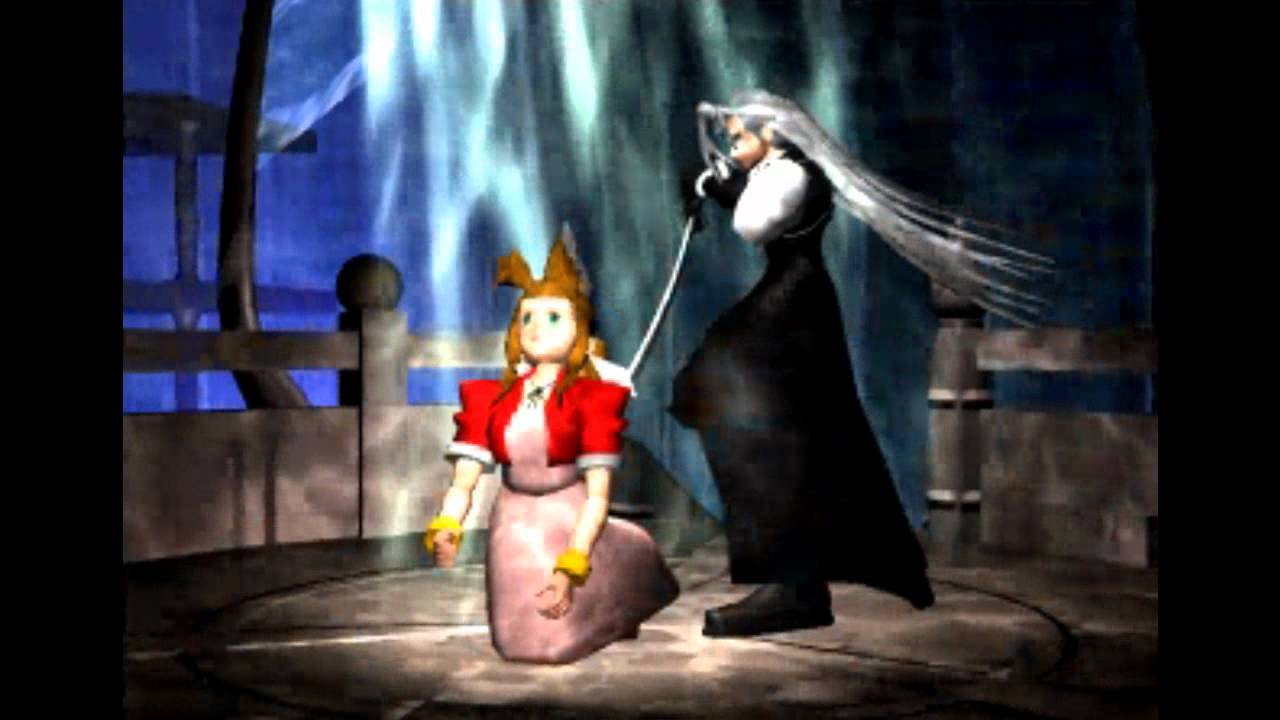
\includegraphics[width=90mm]{maxresdefault.jpg}
\caption{Final Fantasy 7 Aerith Death Cutscene \label{overflow}}
\label{fig:FF7}
\end{figure}
Clearly, the ability to invoke emotion is not something that can be measured using surface roughness or other such technical metrics. Storytelling is an essential aspect in creating an immersive experience. However, there are many games without plots that also offer a highly immersive experience for players. One such game is Minecraft, which offers players a 3d sandbox environment in which they must survive in a hostile world while building and exploring a procedurally generated voxel world containing caves mountains and countless other environments. This game features relatively primitive shaders and lighting effects and has a very minimal plot and few NPCs, yet the game still offers a highly immersive and addictive player experience. Players denote thousands of hours to building detailed and complex structures within the game world and express genuine stress and unease when faced with the in-game monsters, despite their unrealistic appearances. \cite{fig:MCmonster} 
\begin{figure}[ht!]
\centering
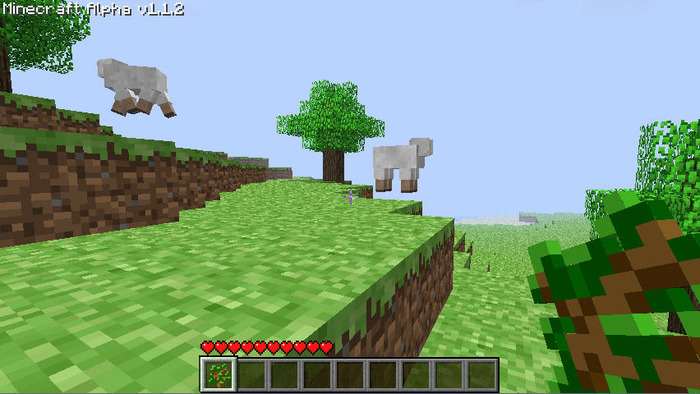
\includegraphics[width=90mm]{minecraft-32.jpg}
\caption{Minecraft Gameplay \label{overflow}}
\label{fig:Minecraft}
\end{figure}
\cite{fig:MCmonster} 
\begin{figure}[ht!]
\centering
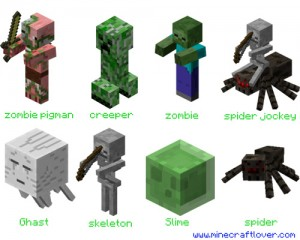
\includegraphics[width=90mm]{minecraft-spider-300x240.jpg}
\caption{Minecraft Hostile NPCs (source: http://www.minecraftlover.com) \label{overflow}}
\label{fig:MCmonster}
\end{figure}
A game's capacity to elicit an emotional response in the user is an essential and undeniable factor in its immersive qualities. We see this in \cite{Brown04agrounded}, where the authors found that the "extent to which a person’s cognitive and
perceptual systems are tricked into believing they are
somewhere other than their physical location" \cite{Brown04agrounded}  was correlated with how well the game's plot and interface conspired to put the agent directly into to the shoes of the character they controlled in the world. A game with strong immersion offers the player with a sense of presence within the game world. In \cite{Brown04agrounded}, the authors note that "The barriers to presence are empathy and atmosphere.
Empathy is the growth of attachment and atmosphere the
development of game construction. Empathy is distinct
from attachment in that you feel attached to a main
character or team but do not necessarily empathize with
their situation. Gamers who did not feel total immersion
talked of lack of empathy and the transfer of consciousness Both these factors are highly dependent on the ability to invoke emotion in the player. However, this does necessitate the existence of non-player characters for the player to talk and otherwise interact with, a game can cause emotional response in the user by properly situating a player within a game environment. A user who feels is playing a game that makes  them feel like they are right there in their character's body is highly immersed with the game world. This particular issue of immersion will be our primary area of investigation moving forwards in this section.
\subsection{The Stoic Conception of Emotion }
	Emotions are an essential aspect of experience. The ancient Greek stoics held that the soul of a human (\textit{pneuma psychikon}) was a mixture of the elements of air and fire. According to the  Hellenistic philosopher Chrysippus,
this elemental mixture forms a breath-like substance called \textit{pneuma}.  Different activities of this substance caused us to have our different cognitive faculties. Stoics held that the pneuma permeating the body of a human  was a portion of the divine pneuma permeating and directing the cosmos. Human souls are a portion of God within us, both animating us and providing us with our reason and intelligence. In contrast to Cartesian dualism, the Stoics held that the soul is a bodily substance. Despite believing the soul is a body, the Stoic conception of the soul is not materialist. Stoic philosophy clearly distinguishes matter from soul. \cite{gould2012the} Stoic philosophers hold a cognitive theory of emotion, which places emphasis on the role of belief and intention in shaping emotional reactions. The classical stoic view holds that emotions express "natural patterns of human functioning and development." \cite{goldie2010the} Stoic philosophers believe that emotion is a subcategory of motivation with respect to human psychology. For the ancient stoic philosophers, motivation was not defined in terms of perception, belief or desire but rather in terms of appearance, impression and impulse. In contrast to contemporary mainstream psychology, the ancient Stoics believe that humans and other animals are naturally drawn to objects and actions that benefit their constitution. Emotions (such as anger, grief, joy) in the Stoic tradition each have a distinctive value and temporal component. For instance, joy was thought to be correlated with good in the future while fear was associated with bad in the future. Stoics see adult human motivation has having the unique characteristic of rationality. However, the defining characteristic of an emotion under the Stoic account is "assent to the rational impression that it is appropriate to react in a certain way to a give situation." \cite{goldie2010the}
Ancient Stoics view emotions as subset of the types of motivations that adult human agents experience.
\subsection{Phenomenology and Emotions}
First posited by Edmund Husserl in the 1900s, phenomenology has been highly influential in fields of philosophy of mind and psychology. Husserl's Phenomenology seeks to establish a radical new first science focused on the study of structures of consciousness as experienced from the first-person perspective. Phrenologists hold that the central structure of an experience is its intentionality. In the philosophy of mind, a mental state or experience is said to be intentional if it is \textit{about} something. This "aboutness" can arise from an experience or mental state's content or from its role as an abstract representation of a particular, idea, or class of particulars or ideas.  Phenomenology differs greatly between theorists. In classical Husserlian phenomenology, our experience represents  
\section{Subconscious Emotion and Immersion}
\subsection{Introduction}
In this section, we shift tack and investigate empirically whether subconscious emotional responses to phenomena in VR environments correlate with an agent's evaluation of said environment as immersive. To do this, we need to investigate the subjective experience of an event feeling real.  To do this, we will use ideas from Stoicism and Phenomenology, two schools of philosophical thought with distinctive views on the status of emotions. 
\subsection{Methods}
\subsubsection{Participants}
Participants were $N$ college students enrolled in philosophy and computer science courses who volunteered via surveys sent out to the departmental list serves. Students were also solicited to volunteer for the experiment in several undergraduate computer science and philosophy classes geared towards first and second-year students.
\subsubsection{Procedure}
Test subjects will be asked to complete a short survey prior to enter the virtual space. The survey questions are listed below: \begin{enumerate}
	\item Have you ever experienced Virtual Reality before? If so, briefly describe your experience?
	\item On a scale of 1 to 10 (with ten being the highest), how freighted are you of heights? 
		\item On a scale of 1 to 10 (with ten being the highest), how freighted are you of enclosed or small spaces?
	\item How frequently do you play video games? Would you describe yourself as a novice, experienced or "hardcore" gamer? 
	\item  On a scale of 1 to 10 (with ten being the highest), how freighted are you of spiders?
		\item  On a scale of 1 to 10 (with ten being the highest), how freighted are you of clowns?
			\item  On a scale of 1 to 10 (with ten being the highest), how freighted are you of cockroaches?
\item What gender do you identify as?
\end{enumerate}
The purpose of the study shall be described to the user and in the event of a strong answer (>8) either question 2 or 3, the user will be advised not to participate in the aspects of the project that might trigger their fear of heights or claustrophobia. Questions 5, 6 and 7 are dummy questions designed to ensure that players will receive prior notice of the experiment variables.  Users shall then be introduced to the HTC Vive hardware. Each component of the system shall be briefly explained and the player will have the opportunity to walk around in small clearing area in order to learn how to perform the following tasks within the VR space. First, the player shall be shown how to move and teleport around the virtual space. Next, the player shall be shown how to grasp items within the virtual world. Finally, the player will be shown how climb objects using the HTC Vive's motion tracking wands. Having shown the player how to leverage the various features of the hardware, the test coordinator will direct the player to complete a series of in game tasks. After completion of the scenario or task, the player will be asked to take a second survey. Descriptions of the player tasks are located in table \ref{table:tasks}. Descriptions of the survey questions are located in table \ref{table:questions}.

\begin{table}
	\begin{center}
\begin{tabular}{l p{8cm}}
\textbf{Task} & \textbf{Explanation}  \\
Climbing the rope & In this section of the experiment, users will be asked to navigate to and climb a rope hanging alongside a mountain. The rope is attached to a beam which juts out of the mountain and over a body of water. Upon reaching the top of the rope. The user will have to use a series of highlighted climbing to affordances to reach the top of the beam. This task is designed to force the user to experience the feeling of being atop a great height and to cause the user to feel insecure at a height due to the non-static nature of the rope and other affordances. \newline  \\
Escape the trash compactor! & Inspired by the classic trash compactor scene in \textit{Star Wars: Episode IV A New Hope}, the player must use their arms to prevent the side walls of a narrow enclosed space from crushing them while attempting to make their way to the door at the other end of the door. Unless actively being touched by the player, the side walls of the space will move towards the center of the room. The player will be forced to circumnavigate a series obstacle which may require either the remove of debris or the placement of debris objects at a particular point in order to progress. \newline \\
Buried alive & Upon pressing a button, the player will be covered in a large quantity of small sphere objects. The player will be forced to push them off of their face and out of their way in order to progress through the confined spaces in this maze-like tunnel. A large very visible timer will count down the amount of oxygen the player character has left.
\label{table:tasks}
\end{tabular}
\end{center}
	\caption{User Tasks}
	\caption*{
		A legend, even a table can be used

	}


\end{table}
Throughout each task, timers and motion and location trackers will be used to collect data about the player's actions. These collection systems will begin tracking the player when he or she's avatar passes through a specific set of coordinates on the map. The results of each test are stored as a row in a comma separated value (CSV) spreadsheet upon the conclusion of the test. A description of each capture point is provided below:
\begin{enumerate}
	\item \textbf{Climbing the Rope} \begin{enumerate}
		\item Once the player attaches himself or herself to the rope (by squeezing the side buttons on the Vive wand), the system will begin tracking the number of milliseconds which pass until the Wand is unattached from the rope. Since moving up or down a rope on the Vive requires the player to detach and move up or down their hands, this test will measure the player's reluctance to risk movement on the rope. The system will also record the X, Y and Z coordinates of the player at the each rope grip event.
	\item Teleportation events will also be recorded by the system. This will allow us to see whether the player decides to leverage the game's teleport ability in order to skip frightening portions of the test. The system will record the X, Y and Z coordinates of the player at the time of a teleport event and where they teleport to.
	\item Falls will also be recorded. Anytime the player is in freefall for more then 30 milliseconds, the duration of the fall will be recorded in the CSV.
	\item Finally, the overall time between the start of the test and the player reaching the summit (the end point designated by the testing supervisor) will be measured.	
\end{enumerate}
\item \textbf{Escape the Trash Compactor}   \begin{enumerate}
	\item The amount of time taken by the player to reach the door of the room will be measured in this test.
	\item Several photos of Wooster buildings and other familiar objects which do not conform to the  environment of the room are located in the debris the player must traverse. Upon completion of the event, the player will be asked whether these objects were inside the environment via a short survey.
\end{enumerate}
\item \textbf{Buried alive} \begin{enumerate}
	\item The total amount of time the player spends escaping will be measured. 
\end{enumerate}
\end{enumerate}
%Measuring immersion requires an understanding of the subjective experience of playing a game or experiencing a VR environment. This sort of data cannot be truly captured by quantitative methods alone. Phenomenology offers the perfect means for understanding the experience of playing games. We will use methodologies form Phenomenological social studies in order to better understand the experience of playing a game. In order to understand the person or persons she is studying, social scientists argue that a researvher must grasp what phenomenologists call 'meaning structure'. The phenomenological conception of s to the web of meanings that are mutually constituted. Meanings, in other words, come in structures and attain meaning in relation to other meanings, not in isolation. This process of meaning constitution is largely a social process, which means that the researcher who is interested in this must study it when people interact. \begin{enumerate}
 	\item 
 \end{enumerate}
